\usepackage{amsthm}

\newtheorem{theorem}{Theorem}[chapter]
\newtheorem{lemma}           [theorem] {Lemma}   
\newtheorem{folg}           [theorem] {Folgerung}   

\newtheorem{frage}       [theorem] {Frage}   
\newtheorem{question}       [theorem] {Question}   
\newtheorem{aufgabe}       [theorem] {Aufgabe}   
\newtheorem{exercise}       [theorem] {Exercise}  

\newtheorem{proposition}     [theorem] {Proposition}  
\newtheorem{satz}     [theorem] {Satz}  
\newtheorem{fact}{Fact}
\newtheorem{definition}      [theorem] {Definition} 

\theoremstyle{definition} 
\newtheorem{bemerkung}     [theorem] {Bemerkung}  
\newtheorem{beispiel}       [theorem] {Beispiel}  
\newtheorem{example}       [theorem] {Example}  
\newtheorem*{example*} {Example}  
\newtheorem{notation}       [theorem] {Notation}  
\newtheorem*{Faust}[theorem]{Rule of Thumb}
\newtheorem*{Boxx}[theorem]{Concept}

%\subsection*{Image and preimage}

For every well-defined map $f: X\to Y$ and $A\subset X$, $B \subset Y$ we are interested in the following sets:
\begin{Definition}{} 
Let $f: X\rightarrow Y$ be a function and $A\subset X$ and $B\subset Y$ some sets.

$$f(A):= \{ f(x): x\in A\}$$ 
is called the \emph{image} of $A$ under $f$.

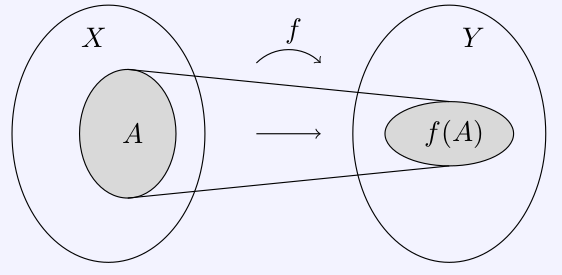
\includegraphics{./image.png}
 
$$f^{-1}(B):= \{ x\in X: f(x) \in B \}$$ is called the \emph{preimage} of $B$ under $f$.
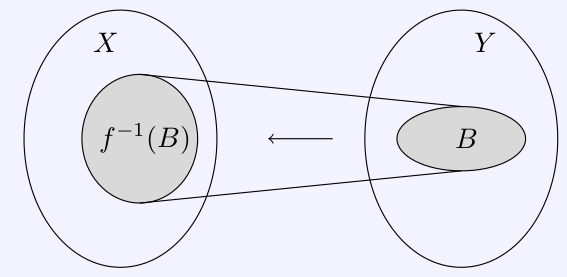
\includegraphics{./preimage.png}

\end{Definition}
%
Note that the preimage can also be the empty set if none of the
elements in $B$ are ``hit'' by the map.

To describe the behaviour of a map,
the following sets are very important:

\begin{Definition}[Range and fiber]
Let $f: X\rightarrow Y$ be a map. Then
\begin{align*}
 \mathrm{Ran}(f) &:= f(X) = \{ f(x) : x \in X \} 
\end{align*}
is called the \emph{range} of $f$.
For each $y\in Y$ the set
\begin{align*}
 f^{-1}(\{y \}) &:= \{ x \in X : f(x) = y \} 
\end{align*}
is called a \emph{fiber} of $f$.
\end{Definition}
